%%%%%%%%%%%%%%%%%%%%%%%%%%%%%%%%%%%%%%%%%%%%%%%%%%%%%%%%%%%%%%%%%%%%%
%% This is a (brief) model paper using the achemso class
%% The document class accepts keyval options, which should include
%% the target journal and optionally the manuscript type.
%%%%%%%%%%%%%%%%%%%%%%%%%%%%%%%%%%%%%%%%%%%%%%%%%%%%%%%%%%%%%%%%%%%%%
\documentclass[journal=jacsat,manuscript=article]{achemso}

%%%%%%%%%%%%%%%%%%%%%%%%%%%%%%%%%%%%%%%%%%%%%%%%%%%%%%%%%%%%%%%%%%%%%
%% Place any additional packages needed here.  Only include packages
%% which are essential, to avoid problems later. Do NOT use any
%% packages which require e-TeX (for example etoolbox): the e-TeX
%% extensions are not currently available on the ACS conversion
%% servers.
%%%%%%%%%%%%%%%%%%%%%%%%%%%%%%%%%%%%%%%%%%%%%%%%%%%%%%%%%%%%%%%%%%%%%
\usepackage[version=3]{mhchem} % Formula subscripts using \ce{}
\usepackage{amsmath}
\usepackage{subcaption}
\usepackage{gensymb}

%%%%%%%%%%%%%%%%%%%%%%%%%%%%%%%%%%%%%%%%%%%%%%%%%%%%%%%%%%%%%%%%%%%%%
%% If issues arise when submitting your manuscript, you may want to
%% un-comment the next line.  This provides information on the
%% version of every file you have used.
%%%%%%%%%%%%%%%%%%%%%%%%%%%%%%%%%%%%%%%%%%%%%%%%%%%%%%%%%%%%%%%%%%%%%
%%\listfiles

%%%%%%%%%%%%%%%%%%%%%%%%%%%%%%%%%%%%%%%%%%%%%%%%%%%%%%%%%%%%%%%%%%%%%
%% Place any additional macros here.  Please use \newcommand* where
%% possible, and avoid layout-changing macros (which are not used
%% when typesetting).
%%%%%%%%%%%%%%%%%%%%%%%%%%%%%%%%%%%%%%%%%%%%%%%%%%%%%%%%%%%%%%%%%%%%%
\newcommand*\mycommand[1]{\texttt{\emph{#1}}}

%%%%%%%%%%%%%%%%%%%%%%%%%%%%%%%%%%%%%%%%%%%%%%%%%%%%%%%%%%%%%%%%%%%%%
%% Meta-data block
%% ---------------
%% Each author should be given as a separate \author command.
%%
%% Corresponding authors should have an e-mail given after the author
%% name as an \email command. Phone and fax numbers can be given
%% using \phone and \fax, respectively; this information is optional.
%%
%% The affiliation of authors is given after the authors; each
%% \affiliation command applies to all preceding authors not already
%% assigned an affiliation.
%%
%% The affiliation takes an option argument for the short name.  This
%% will typically be something like "University of Somewhere".
%%
%% The \altaffiliation macro should be used for new address, etc.
%% On the other hand, \alsoaffiliation is used on a per author basis
%% when authors are associated with multiple institutions.
%%%%%%%%%%%%%%%%%%%%%%%%%%%%%%%%%%%%%%%%%%%%%%%%%%%%%%%%%%%%%%%%%%%%%
\author{Elliott Capek}
\affiliation{Department of Biochemistry, Oregon State University}
\email{capeke@oregonstate.edu}
\phone{(971) 207 8193}
\author{Hassan Alnatah}
\author{Laikana Ly}
\author{Joey Orton}
%% \alsoaffiliation[]{}
\author{Aidan Estelle}
%% \affiliation{Department of Biochemistry, Oregon State University}

%%%%%%%%%%%%%%%%%%%%%%%%%%%%%%%%%%%%%%%%%%%%%%%%%%%%%%%%%%%%%%%%%%%%%
%% The document title should be given as usual. Some journals require
%% a running title from the author: this should be supplied as an
%% optional argument to \title.
%%%%%%%%%%%%%%%%%%%%%%%%%%%%%%%%%%%%%%%%%%%%%%%%%%%%%%%%%%%%%%%%%%%%%
\title[]{Exploring the role of electric field in the catalase active site}

%%%%%%%%%%%%%%%%%%%%%%%%%%%%%%%%%%%%%%%%%%%%%%%%%%%%%%%%%%%%%%%%%%%%%
%% Some journals require a list of abbreviations or keywords to be
%% supplied. These should be set up here, and will be printed after
%% the title and author information, if needed.
%%%%%%%%%%%%%%%%%%%%%%%%%%%%%%%%%%%%%%%%%%%%%%%%%%%%%%%%%%%%%%%%%%%%%
\keywords{Catalase, noncanonical amino acid, active site, channel flow}

\begin{document}
%%%%%%%%%%%%%%%%%%%%%%%%%%%%%%%%%%%%%%%%%%%%%%%%%%%%%%%%%%%%%%%%%%%%%
%% The manuscript does not need to include \maketitle, which is
%% executed automatically.  The document should begin with an
%% abstract, if appropriate.  If one is given and should not be, the
%% contents will be gobbled.
%%%%%%%%%%%%%%%%%%%%%%%%%%%%%%%%%%%%%%%%%%%%%%%%%%%%%%%%%%%%%%%%%%%%%
\begin{abstract}
  Catalase is a diffusion-limited enzyme, and thus has optimized the rates of each step in its interaction with substrate. Recent evidence suggests that one such optimization is the use of an electric field in the active site to orient substrates for ideal reaction with catalytic residues. Here we study the role of electric field in the catalytic active site by introducing minor electric purturbations through genetic code expansion. Initial results indicate that the incorporation of noncanonical polar residues into the active site does not destroy function. More work is needed to fully determine the influence of electric field in the active site.\\
\end{abstract}

%%%%%%%%%%%%%%%%%%%%%%%%%%%%%%%%%%%%%%%%%%%%%%%%%%%%%%%%%%%%%%%%%%%%%
%% Start the main part of the manuscript here.
%%%%%%%%%%%%%%%%%%%%%%%%%%%%%%%%%%%%%%%%%%%%%%%%%%%%%%%%%%%%%%%%%%%%%
\section{Introduction}
%% Catalase is an enzyme which catalyzes the breakdown of hydrogen peroxide into water and oxygen gas. This is an important detoxification reaction, since hydrogen peroxide is a reactive toxin generated by several biological processes. Catalase is a tetrameric protein which uses a heme group in its active site to facilitate the breakdown of hydrogen peroxide. The molecular mechaninism of catalase proceeds in two steps. First, the heme reduces a hydrogen peroxide, producing water and the so-called Cpd I. Then Cpd I oxidizes a second hydrogen peroxide, producing water and oxygen gas. This second step is mediated by a histidine near the active site \cite{alfonso-prieto}.

%% Catalase's activity is nearly diffusion-limited \cite{kcatkm, difflimit}. This rate suggests that nearly every step in the substrate-enzyme interaction is optimized for speed. Understanding the optimizations of diffusion-limited proteins can provide many insights into how proteins achieve their functions. Catalase has a variety of interesting quirks for funneling substrate into its active pocket. The enzyme has a number of high-H2O2-residency surface residues near its active channel, which are believed to concentrate the substrate near the entrance to the active channel \cite{concentrateh2o2}. The active channel itself seems optimized to maximize substrate flow, to the point that mutagenesis to open the channel decreases enzyme activity \cite{substrateflow}. The channel seems to be capable of selecting the molecules which enter it using a patch of hydrophobic residues which are situated to preferentially pass the bulkier H2O2 \cite{molecularruler}. Even the directionality of substrate within the channel seems to be controlled: one channel is used for substrate entrance, and the other for product exit \cite{lateralchannel}. An new finding suggests that catalase might control not just the presence of hydrogen peroxide, but even its orientation as it enters the active site. It is believed that an electric field from a negative Asn residue to the positive heme acts to orient the H2O2 dipole, positioning the molecule such that it enters the active site at an angle ideal for reacting \cite{electricpotential}. This use of an electric field over a long range to create an ``orienting field'' is a new and exciting usage of residues to achieve a function; understanding its role in catalase may help to understand the mechanisms of other proteins.

%% In this study we hope to study the proposed orienting field optimization and its influence on catalase activity. In particular, we hope to carefully disrupt the wildtype active site potential environment by introducing a new charged residue, then examine the effect this disruption has on activity. For meaningful results, we must be careful to not introduce structural modifications to the enzyme. To ensure this, we will use genetic code expansion to incorporate 3-nitrotyrosine in place of tyrosine 206. The T206NY mutation will add only 30 $\AA^3$ of steric bulk \cite{3ntsize}, so should have minimal influence on active site structure. The theorized results of this addition are diagrammed in Figure \ref{fig:hypothesis}. To study the influence of field disruption on activity, we will study the activity of T206NY above and below its pKa of 6.8 \cite{3ntsize}. Wildtype catalase activity is constant under pH values from 5 to 10 \cite{phdependence,kcatkm}, so pH-dependence should only be seen if electric environment in the active site is important for activity.\\

Catalase is an enzyme which catalyzes the breakdown of hydrogen peroxide into water and oxygen gas. This is an important detoxification reaction, since hydrogen peroxide is a reactive toxin generated by several biological processes. Catalase is a tetrameric protein which uses a heme group in its active site to facilitate the breakdown of hydrogen peroxide. The molecular mechaninism of catalase proceeds in two steps. First, the heme reduces a hydrogen peroxide, producing water and the so-called Cpd I. Then Cpd I oxidizes a second hydrogen peroxide, producing water and oxygen gas. This second step is mediated by a histidine near the active site \cite{alfonso-prieto}.\\

One remaining question about catalase is how it achieves its remarkable speed given its buried active site. The enzyme is nearly diffusion-limited\cite{kcatkm, difflimit}, indicating it turns substrate to product at close to the optimal rate. However, in order to reach the active site, hydrogen peroxide must diffuse through a 30 $\AA$ tunnel\cite{substrateflow}. Thus, substrate must be transported very efficiently through the protein. Understanding how this transport process works could provide lots of insight into how enzymes traffic substrate into buried active sites. Catalase is one of the most studied proteins in existence, and so represents a good model protein for understanding substrate trafficking.\\

Previous work on substrate trafficking has illuminated various stages in the process. The enzyme has a number of high-H2O2-residency surface residues, which are believed to concentrate the substrate near the entrance to the active channel \cite{concentrateh2o2}. The active channel itself seems optimized to maximize substrate flow, to the point that mutagenesis to open the channel decreases enzyme activity \cite{substrateflow}. The channel seems to be capable of selecting the molecules which enter it using a patch of hydrophobic residues which are situated to preferentially pass the bulkier H2O2 \cite{molecularruler}. Even the directionality of substrate within the channel seems to be controlled: one channel is used for substrate entrance, and the other for product exit \cite{lateralchannel}. However, how substrate is traficked once in the active site antechamber is still an open question.\\

One tool proteins are known to use to speed up active site kinetics is the use of electric fields. Superoxide dismutase is known to have a strong E-field in its active site to stabilize dipolar intermediates \cite{conserved-as-efield-sod, concentrated-as-efield-sod}. Several other proteins are known to use a similar effect \cite{efield-review} (be more precise here). It has been suggested that catalase uses an electric field in its active site to orient and traffick hydrogen peroxide to its active heme \cite{electricpotential}. This model, proposed by Chelikani \textit{et. al}, theorizes that a strong electric field from the negative asparigine 181 at the top of the active site antechamber extends to the strongly positive heme iron, as shown in Figure \ref{fig:hypothesis}.d. This electric field would orient incoming hydrogen peroxides in the optimal rotation for reaction with heme.\\

An issue with mutagenesis studies like Chelikani \textit{et. al.} is that catalase's active site is very sensitive to changes. Mutagenesis of many residues results in large changes in enzyme kinetics \cite{substrateflow}. Here we conduct a less invasive experiment to probe the role of electric field in the catalase active site. We use genetic code expansion \cite{hammill} to incorporate two functional groups onto F206 in the catalase active site, turning it into 3-nitrotyrosine (Figure \ref{fig:hypothesis}.e). This change is important because it a.) is tiny, adding only 30 $\AA^3$ of steric bulk \cite{3ntsize}, and b.) incorporates a hydroxy group of pKa 7.0 into the catalase active site \cite{3ntsize}. Catalase activity is pH-invariant in the range of 5 to 9 \cite{phdependence,kcatkm}; thus, by incorporating a group which gains charge at pH 7, we can precisely study the effect of charge in the catalase active site on enzyme kinetics without worrying about the undesired effects of mutagenesis.\\

\begin{figure}
  \begin{subfigure}{0.49\textwidth}
    \begin{minipage}{0.1\textwidth}\caption{}\end{minipage}%
    \begin{minipage}{.9\textwidth}
      %% \includegraphics[width=0.5\linewidth]{figures/cartoon-visualization.png}%
      \includegraphics[width=\linewidth]{figures/channel-visualization.png}
    \end{minipage}
  \end{subfigure}
  \begin{subfigure}{0.5\textwidth}
    \begin{minipage}{0.1\textwidth}\caption{}\end{minipage}%
    \begin{minipage}{.9\textwidth}
      \includegraphics[width=0.5\linewidth]{figures/active-site-visualization.png}%
      \includegraphics[width=0.5\linewidth]{figures/active-site-visualization.png}%
    \end{minipage}
  \end{subfigure}
  \caption{Depiction of catalase active pocket. \textbf{Left:} wildtype pocket with proposed ligand-orienting E-field \cite{electricpotential}. The field should orient H2O2 for optimal reaction with the heme. \textbf{Right:} modified HPII-3NY with a deprotonated 3-nitrotyrosine residue at site 206, with hypothetical augmented E-field. The disrupted E-field should result in un- or mis-aligned substrate.}
  \label{fig:hypothesis}
\end{figure}

\section{Methods}
\textbf{Protein production}\\
Wildtype protein was expressed by transforming the plasmid pBad-HPII (Fig \ref{fig:protein-design}.b, modified from Addgene ID 105839), containing WT HPII gene, into competent \textit{E. coli} DH10B cells via heat-shock. pBad-HPII plasmid includes ampicillin resistance, an arabinose-induced promoter, and a 6xHis codon sequence on the N-term of the HPII gene. Cells were then grown in autoinduction media with an arabinose inducer (0.1\% aspartate, 0.2\% glycerol, 100$\mu g / mL$ ampicillin, mineral salts, 0.05\% glucose, 20mM MgSO4, 0.05\% arabinose, trace metals and amino acid mix, pH 7.5) for 48 hours, shaking, at 37\degree C. Cells were then pelletized and stored at -80\degree C.\\

The same protocol was followed for the ncAA mutant catalases HPII-3NY and HPII-pAzF, except using protein plasmids pBad-HPII-3NY and pBad-HPII-pAzF (Addgene ID 105846) instead. ncAA tRNA synthase plasmids pDule-Nitro-RS and pDule-pCNF-RS (Fig \ref{fig:protein-design}.b, modified from Addgene ID 85498), which contain a tetracycline resistance gene, a TAG tRNA, and a compatible tRNA synthase, were also transformed into DH10B. ncAA autoinduction media was supplemented with $25\mu g / mL$ tetracycline to select for both plasmids.\\

$OD_{600}$ measurements of cultures at 48 hours growth time were 0.65, 0.58 and 0.45 optical density for HPII, HPII-3NY and HPII-pAzF expressions.\\

\textbf{Protein purification}\\
Pelletized cells were reconstituted in TALON equilibration buffer (50mM sodium phosphate, 300mM NaCl, pH 7.0) and microfluidized, also in equilibration buffer. Lysed cells were spun down at 15K RPM for 20 minutes at 4\degree C. Supernatant was collected and combined with 300$\mu L$ bed volume TALON beads per 100mL cultured cells. TALON-supernatant mix was nutated for 30 minutes at 4\degree C. Bound beads were then spun down at 500g for 5 minutes and the supernatant discarded. The beads were applied to a pre-washed gravity-flow column at room temperature and washed twice with 10mL equilibration buffer. Elution was done using 2mL elution buffer (50mM sodium phosphate, 300mM NaCl, 250mM imidazole, pH 7.0) into four 500$\mu L$ aliquots. Protein was then stored at 4\degree C.\\

\textbf{Concentration determination}\\
A Bio-Rad Bradford assay kit was employed using the standard protocol. Bovine serum albumin was used as the reference protein to construct the standard curve. Concentrations from 125 $\mu g / mL$ to 2 mg/mL were explored. Samples were incubated with dye in cuvettes for 5 minutes at room temperature. Samples were then analyzed via spectrophotometer at 595 \textit{nm} and used to create the standard curve. HPII protein samples were then compared to this standard curve to estimate their concentration.\\

\textbf{Activity assessment}\\
Enzyme velocity was measured using a Vernier Gas Pressure Sensor. Reaction buffer (50mM sodium phosphate, 300mM NaCl, 5\% $H_2O_2$ pH modulated to 5.5, 6.25, 7.0, 7.75, 8.5 via addition of HCL or NaOH) was combined with enzyme (25 $\mu g/mL$, 50 $\mu g/mL$, 50$\mu g/mL$ for HPII, HPII-3NY, HPII-pAzF) to a total volume of $3mL$ in pressure sensor tube. Tubes were sealed and pressure was monitored at 1s intervals for 120 seconds. Data was collected using Vernier LoggerPro.\\

\textbf{pH-dependent assay}\\
pH assays were conducted using the same kinetic method described above. Reactions occured in 3mL equilibration buffer (50mM sodium phosphate, 300mM NaCl, 5\% $H_2O_2$ pH modulated to values from 5 to 10 via addition of HCL or NaOH). On addition of 43$\mu g$ protein, the tubes were mixed and incubated at RT for five minutes, then brought to 5\% $H_2O_2$ and added to pressure assay mechanism. Trials were conducted in triplicate.\\

\section{Results}
%% to add: Chemical nature and location of your ncAAs in the structure. (This might fit best in results).
Noncanonical amino acids (ncAAs) were incorporated into protein constructs by mutating the desired codon to TAG, then adding TAG-recognizing ncAA-tRNA synthetases and compatible tRNAs to cells. His-tagged protein constructs were grown in DH10 \textit{E. coli} and purified using TALON metal affinity resin. An SDS-PAGE gel of purified protein is shown in Figure \ref{fig:pure-gel}. HPII is expected to be in its 84-kD monomeric state in the denaturing and reducing conditions of SDS-PAGE; an 80kD band is seen for all three purified HPII constructs. This verifies that HPII-ncAA cells properly produce noncanonical aminoacyl-tRNA, which is the only tRNA which recognizes the TAG codon and allows for full-length protein translation. Contaminant bands in the gel are faint but visible, suggesting protein of $\approx$ 90\% purity. ncAA-incorporated proteins were grown with and without ncAA to verify proper incorporation. Without ncAA, cells should lack any aminoacyl-tRNA for the TAG codon, and thus HPII-ncAA peptides should stall on the ribosome, resulting in truncated peptides of approximately 22kD. This is seen in Figure \ref{fig:pure-gel}, where HPII-ncAA lanes lacking ncAA lack a 80kD band but do have bands of approximately 25kD.\\

\begin{figure}[h!]
  \centering
  \begin{subfigure}{0.49\textwidth}
    \begin{minipage}{0.1\textwidth}\caption{}\end{minipage}%
    \begin{minipage}{0.9\textwidth}\includegraphics[width=0.9\linewidth]{figures/gene-diagram}\end{minipage}
  \end{subfigure}
  \begin{subfigure}{0.49\textwidth}
    \begin{minipage}{0.1\textwidth}\caption{}\end{minipage}%
    \begin{minipage}{0.9\textwidth}\includegraphics[width=0.9\linewidth]{figures/plasmid-diagram}\end{minipage}
  \end{subfigure}
  \vspace{2mm}
  \begin{subfigure}{\textwidth}
    \centering
    \begin{minipage}{0.1\textwidth}\caption{}\end{minipage}%
    \begin{minipage}{0.9\textwidth}\centering\includegraphics[width=0.7\linewidth]{figures/pure-gel}\end{minipage}
  \end{subfigure}
  \caption{\textbf{Electrophoresis gel of crude lysate and purified protein expression.} \textbf{a.} Gene constructs used. \textbf{b.} Plasmid schematics for relevant plasmids. Amp$^R$ and Tet$^R$ are antibiotic resistance genes, Nitro-Y-RS and pCNF-RS are tRNA synthases compatible with 3-nitrotyrosine and p-azido-l-phenylalanine, and tRNA$_{CUA}$ is a tRNA compatible with the respective synthase. \textbf{c.}Major band in purification lanes correspond to protein of approximately 80kD, as expected for a catalase single subunit. Crude negative control lanes lack 80kD band, consistent with noncanonical amino acid being necessary for noncanonical protein expression. Crude negative control lanes have smaller protein bands, consistent with truncated protein formation.}
\label{fig:pure-gel}
\end{figure}



%% \begin{figure}[h!]
%%   \centering
%%   \begin{minipage}{.4\textwidth}
%%     \begin{tabular}{lll}
%%       \hline
%%       Sample  & OD590 & mg/mL  \\
%%       \hline
%%       WT        & 2.18 & 2.74\\
%%       %% F206NY    & 0.71 & 0.83\\
%%       %% F206pAzF  & 1.51 & 1.88\\
%%       \hline
%%     \end{tabular}
%%   \end{minipage}
%%   \begin{minipage}{.59\textwidth}
%%     \includegraphics[width=\linewidth]{figures/bradford-standard-curve}
%%   \end{minipage}
%%   \caption{Bradford assay results. \textbf{Left:} Sample absorbance at 590 nm and extrapolated concentration. \textbf{Right:} Bradford standard curve.}
%%   \label{fig:bradford-assay}
%% \end{figure}

%% \begin{figure}[h!]
%%   \centering
%%   \begin{subfigure}{0.29\textwidth}
%%     \begin{minipage}{0.1\textwidth}\caption{}\end{minipage}%
%%   \begin{minipage}{.9\textwidth}
%%     \begin{tabular}{lll}
%%       \hline
%%       Sample  & $K_M$ (M) & kcat ($s^{-1}$) \\
%%       \hline
%%       HPII        & $1.3$ & $2.3x10^6$\\
%%       HPII-3NY    & $1.4$ & $6.9x10^6$\\
%%       HPII-pAzF   & $1.7$ & $2.2x10^5$\\
%%       \hline
%%     \end{tabular}
%%   \end{minipage}
%%   \end{subfigure}
%%   \begin{subfigure}{0.69\textwidth}
%%     \begin{minipage}{0.1\textwidth}\caption{}\end{minipage}%
%%   \begin{minipage}{.9\textwidth}
%%     %% \includegraphics[width=\linewidth]{figures/fake-results.png}
%%   \end{minipage}
%%   \end{subfigure}
%%   \caption{Initial kinetic assay results. \textbf{a.} Final kinetic data extrapolated from Michaelis-Menten plot via linear regression. \textbf{b.} Michaelis-Menten plot of enzyme catalytic ($\pm \sigma^2$).}
%%   \label{fig:bradford-assay}
%% \end{figure}

%% \begin{figure}[h!]
%%   \centering
%%   \begin{subfigure}{\textwidth}
%%     \begin{minipage}{0.1\textwidth}\caption{}\end{minipage}%
%%     \begin{minipage}{0.9\textwidth}\includegraphics[width=0.9\linewidth]{figures/kinetics.png}\end{minipage}
%%   \end{subfigure}
%%   \caption{\textbf{Michaelis-Menten plot of kinetic efficiencies of HPII variants.} Kinetic measurements conducted at 25\degree C using the pressure-based assay defined above.}
%% \label{fig:kinetics}
%% \end{figure}

\begin{figure}[h!]
  \centering
  \begin{subfigure}{\textwidth}
    \begin{minipage}{0.1\textwidth}\caption{}\end{minipage}%
    \begin{minipage}{0.9\textwidth}\includegraphics[width=0.9\linewidth]{figures/wildtype-velocity.png}\end{minipage}
  \end{subfigure}
  \begin{subfigure}{\textwidth}
    \begin{minipage}{0.1\textwidth}\caption{}\end{minipage}%
    \begin{minipage}{0.9\textwidth}\includegraphics[width=0.9\linewidth]{figures/3ny-velocity.png}\end{minipage}
  \end{subfigure}
  \caption{\textbf{pH dependent initial velocities of HPII variants.} Left: HPII catalase Right: HPII-3NY.}
\label{fig:ph-dependent-velocities}
\end{figure}

\subsection{Discussion}

\subsection{Conclusion}

\subsection{References}

%%%%%%%%%%%%%%%%%%%%%%%%%%%%%%%%%%%%%%%%%%%%%%%%%%%%%%%%%%%%%%%%%%%%%
%% The same is true for Supporting Information, which should use the
%% suppinfo environment.
%%%%%%%%%%%%%%%%%%%%%%%%%%%%%%%%%%%%%%%%%%%%%%%%%%%%%%%%%%%%%%%%%%%%%
%% \begin{suppinfo}

%% \end{suppinfo}

%%%%%%%%%%%%%%%%%%%%%%%%%%%%%%%%%%%%%%%%%%%%%%%%%%%%%%%%%%%%%%%%%%%%%
%% The appropriate \bibliography command should be placed here.
%% Notice that the class file automatically sets \bibliographystyle
%% and also names the section correctly.
%%%%%%%%%%%%%%%%%%%%%%%%%%%%%%%%%%%%%%%%%%%%%%%%%%%%%%%%%%%%%%%%%%%%%
\bibliography{references}

%%%%%%%%%%%%%%%%%%%%%%%%%%%%%%%%%%%%%%%%%%%%%%%%%%%%%%%%%%%%%%%%%%%%%
%% The "tocentry" environment can be used to create an entry for the
%% graphical table of contents.
%%%%%%%%%%%%%%%%%%%%%%%%%%%%%%%%%%%%%%%%%%%%%%%%%%%%%%%%%%%%%%%%%%%%%

%% \begin{tocentry}

%% \end{tocentry}

\end{document}


results section mantra:
1 - Explain what you did and then describe what you expected as an outcome
2 - Describe the data and show the dta
3 - Interpret the data

Role of the lateral channel in catalase HPII of Escherichia coli, Loewen
They suggest that the perpendicular channel is the entrance channel and the lateral channel is the exhaust channel, because:
-enlarging the perpendicular channel increases peroxidatic activity
-perpendicular seems optimized for bringin in H2O2
-lateral channel is blocked in some catalases

Substrate Flow, Loewen
There are H2O2 binding sites in the heme distal pocket and main channel
There are several input channels; what are their purposes?
There is a ``molecular ruler'' in the main channel which selects for H2O2 against water
Active site mutations which allow more water in slow down the rxn rate
This paper discusses unidirectional flow of H2O2 through the main channel

Active and inhibited catalase structures, tainer
This is the paper about the hydrophobic ``molecular ruler''
A hydrophobic region distal to the heme cleft contains phenylalanines, tryptophan and two valines
Authors propose that two waters (one h-bonded to human Asn148 and His75; other h-bonded to gln168 and asp128) form a ``ruler''
This ``ruler'' is far enough apart that only H2O2 can stably occupy the distance betweeen, thus allowing only H2O2 to enter, not H2O
This would explain why opening the perpendicular channel decreases the rate

Site-Specific Incorporation of 3-Nitrotyrosine as a Probe of pKa Perturbation of Redox-Active Tyrosines in Ribonucleotide Reductase, Stubbe
pKa of 3NY can vary lots, between 7.5-10

\cite{kcatkm}
Km: 1.1M,
kcat/Km: 6.6*10^7/M/s

possibly make a figure with the h2o2 and water from the electric potential paper?
make inkscape gene block diagram

---------------
Arguments about protein production, validation, and ncAA validation:
We know we have wildtype protein because our gels have bands, indicating protein of the proper size was made with His tags
We know our WT protein was active by quantitative assays

We know our noncanonical protein was expressed because we have lanes in the gel of the proper size. repurposed TAG codon competes with the TAG release factor, meaning we should get some truncated protein, because ours is N-terminally labelled. We don't, which is interesting.



new stuff
---------------------------
Structure of Catalase HPII From Escherichia coli, at 1.9 A˚ Resolution, Bravo + Fita
Describes the channels in HPII
``Channels might be long and narrow to promote the selectivity for H2O2 of HPII''

--Find a way to get the 2 channels: main one (intake? distal?), 590-595 one (lateral?)
